 
\section{Problem 1}
\label{part1}
\begin{verbatim}
The ``friendship paradox'' (http://en.wikipedia.org/wiki/Friendship_paradox)
says that your friends have more friends than you do.  

Determine if the friendship paradox holds for my Facebook
account.* Compute the mean, standard deviation, and median of the
number of friends that my friends have.  Create a graph of the
number of friends (y-axis) and the friends themselves, sorted by
number of friends (x-axis).  (The friends don't need to be labeled
on the x-axis: just f1, f2, f3, ... fn.)  Do include me in the graph
and label me accordingly.

* = This used to be more interesting when you could more easily download
your friend's friends data from Facebook.  Facebook now requires each
friend to approve this operation, effectively making it impossible.

I will email to the list the XML file that contains my Facebook
friendship graph ca. Oct, 2013.  The interesting part of the file looks
like this (for 1 friend):

<node id=``Johan_Bollen_1448621116''>
        <data key=``Label''>Johan Bollen</data>
        <data key=``uid''><![CDATA[1448621116]]></data>
        <data key=``name''><![CDATA[Johan Bollen]]></data>
        <data key=``mutual_friend_count''><![CDATA[37]]></data>
        <data key=``friend_count''><![CDATA[420]]></data>
</node>

It is in GraphML format: http://graphml.graphdrawing.org/
\end{verbatim}

\subsection{Solution}

\begin{enumerate}
\item I tried to understand ``Friendship paradox'' from the source provided in the question.
\item It is the phenomenon which states that your friends on an average will have more friends than you.
\item Based on this phenomenon this question is phrased and the solution proves it.
\item As facebook has increased its privacy settings, we cannot scrap friends details now and so we got XML file from our professor which was previously saved in 2013.
\item Now this file should be processed and I need to get the number of friends my friends have and it compare it with my count of friends.
\item I used minidom to parse the graphml file and Tag name ``data'' was used to get all the data elements with this tag name.
\item Later with the help of key value from the data attributes I managed to get the ``Label'' and ``friend\_count''. 
\item So people with friend\_count are only considered and all of them have been written into a csv file. Python code for this can be found in \ref{lst:q1-1}
\item One csv file consists of all the Labels of friends and their friends count but it does not ``Michael Dr.Nelson's'' friends count. This is shown in \ref{Sample_list1}
\item Other csv file consists of the same data as in previous file but ``Dr.Michael Nelson's'' friend count is included here. This is shown in \ref{Sample list2}
\item The reason for creating to different files is that one with Dr.Nelson's count is used to plot graph and other one without Dr.Nelson's count is used to calculate mean,median and standard deviation.
\item Once I got these two files I wrote code in R to find out mean,median and standard deviation and they are shown in \ref{lst:q1R}.
\item A bar plot is also drawn which shows friends on x-axis and friends count for each friend on y-axis. This can been seen in \ref{graph1} and the code for it can be seen in \ref{2nd:q1R}
\item Friends count of Dr.Michael Nelson is indicated with a blue arrow mark in the graph so that we can visualize the friendship paradox here.
\item The Mean we calculated is 358.987 and the friends count of Dr.Michael Nelson is 154. Therefore friends count of Dr.Michael Nelson is less than the Mean which shows that Michael Nelson's friends have more friends than Michael Nelson. 
\item This proves Friendship Paradox using facebook friends list.

\end{enumerate}

\subsection{Code Listing}
Here is the Python program for acquiring friends and the number of friends they have in facebook. 


\lstinputlisting[language=Python,breaklines = true,frame=single,caption={Python program for acquiring facebook friends and the count of their friends }, label=lst:q1-1,captionpos=b,numbers=left,showspaces=false,showstringspaces=false,basicstyle=\footnotesize]{get_frnds_count.py}
\newpage
\subsection{Results}

\subsubsection{Sample list of Friends and their count without Nelson}
\begin{figure}[ht]    
    \begin{center}
        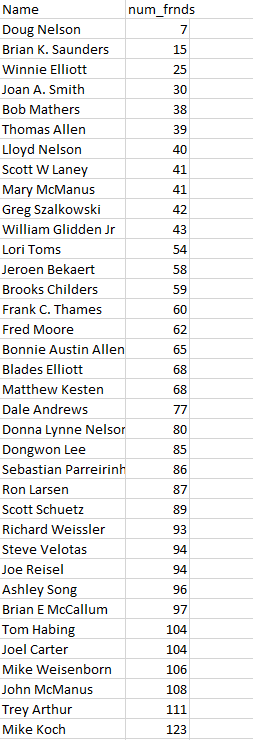
\includegraphics[scale=0.9]{frnds_without_source_fb.png}
        \caption{Sample list of Friends and their count without Nelson}
        \label{Sample_list1}
    \end{center}
\end{figure}
\newpage
\subsubsection{Sample list of Friends and their count with Nelson}
\begin{figure}[ht]    
    \begin{center}
        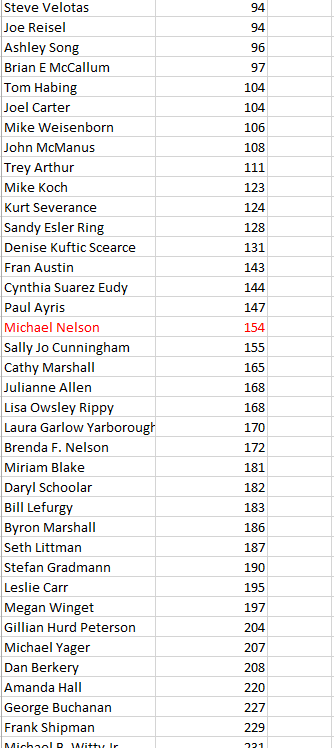
\includegraphics[scale=0.9]{frnds_with_source_fb.png}
        \caption{Sample list of Friends and their count with Nelson}
        \label{Sample list2}
    \end{center}
\end{figure}
\newpage
\subsubsection{R code and results for Calculation of Mean,Median and Standard Deviation}
\lstinputlisting[language=R,breaklines = true,frame=single,caption={R code for Mean,Median and Standard Deviation}, label=lst:q1R,captionpos=b,numbers=left,showspaces=false,showstringspaces=false,basicstyle=\footnotesize]{calculations_fb.R}

\subsubsection{R code and results for plotting graph between facebook friends and their count of friends}
\lstinputlisting[language=R,breaklines = true,frame=single,caption={R code for plotting graph between facebook friends and their count of friends}, label=2nd:q1R,captionpos=b,numbers=left,showspaces=false,showstringspaces=false,basicstyle=\footnotesize]{Rcodeforgraph_fb.R}
\newpage
\subsubsection{Graph showing facebook friends and their count of friends}
\begin{figure}[ht]    
    \begin{center}
        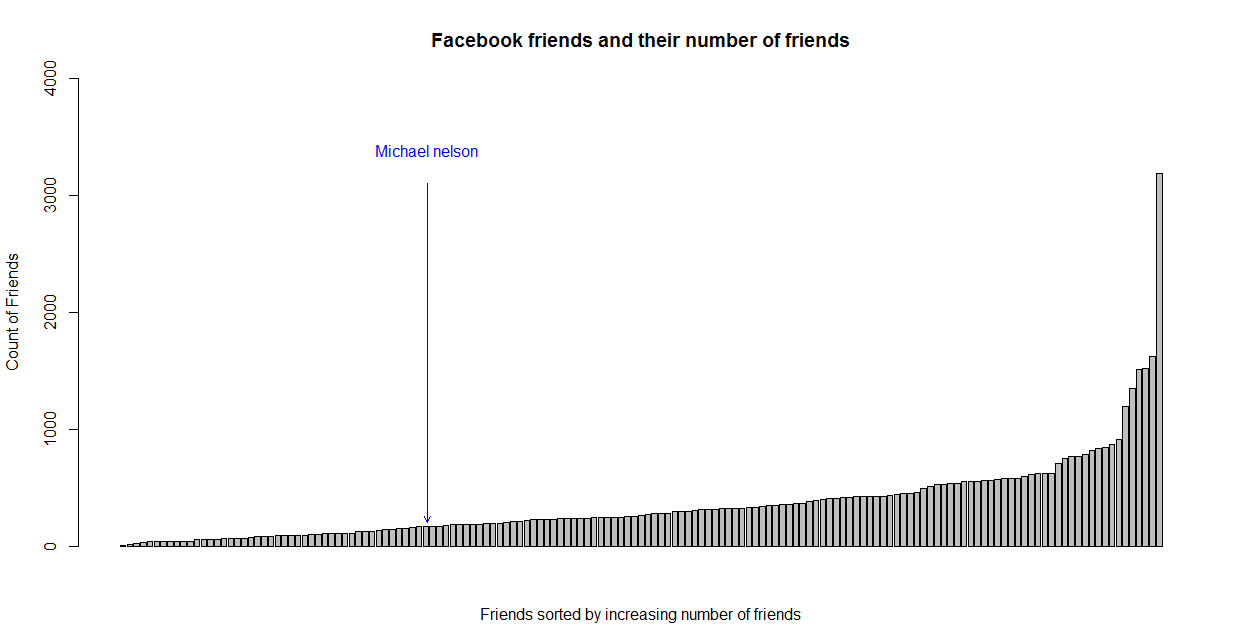
\includegraphics[scale=0.4]{facebookfriendsgraph.png}
        \caption{facebook friends and their count of friends}
        \label{graph1}
    \end{center}
\end{figure}
\newpage